% !TEX TS-program = pdflatex
% !TEX encoding = UTF-8 Unicode
\documentclass[a4paper]{article}
\usepackage[english]{babel}
\usepackage[T1]{fontenc}
\usepackage[utf8]{inputenc}
\usepackage{mathtools}
\usepackage[pdftex]{graphicx}
\usepackage{float}
\usepackage{fancyhdr}
\usepackage{geometry}
\usepackage{booktabs} % for much better looking tables
\usepackage{array} % for better arrays (eg matrices) in maths
\usepackage{paralist} % very flexible & customisable lists (eg. enumerate/itemize, etc.)
\usepackage{verbatim} % adds environment for commenting out blocks of text & for better verbatim
\usepackage{subfig} % make it possible to include more than one captioned figure/table in a single float

%%% HEADERS & FOOTERS

\author{Jonathan Karlsson - jonka293 - 890201-1991 \and Niclas Olofsson - nicol271 - 900904-5338}
\pagestyle{fancy} % options: empty , plain , fancy
\renewcommand{\headrulewidth}{1pt} % customise the layout...
\fancyhead[LO,LE]{Laboration 5 - TDDC78}
\lfoot{}\cfoot{\thepage}\rfoot{}
\setlength{\parindent}{0pt}

%%%% SECTION TITLE APPEARANCE

%\usepackage{sectsty}
%\allsectionsfont{\sffamily\mdseries\upshape} % (See the fntguide.pdf for font help)
%% (This matches ConTeXt defaults)
%
%%%% ToC (table of contents) APPEARANCE
%\usepackage[nottoc,notlof,notlot]{tocbibind} % Put the bibliography in the ToC
%\usepackage[titles,subfigure]{tocloft} % Alter the style of the Table of Contents
%\renewcommand{\cftsecfont}{\rmfamily\mdseries\upshape}
%\renewcommand{\cftsecpagefont}{\rmfamily\mdseries\upshape} % No bold!

%%% END Article customizations

%%% The "real" document content comes below...

\title{Laboration 5 - TDDC78}

%\date{} % Activate to display a given date or no date (if empty),
% otherwise the current date is printed

\begin{document}

\maketitle

\section{TotalView}
The debugger TotalView was pretty complicated to get started with, it required some special setup and such, but when it did start to work then we got a nice looking window with our code. It was pretty intuitive how to use it with clear buttons for single stepping and running the code. We have previously worked with the built in debugger in eclipse and found the interface a bit more crude in TotalView, but it had similar functionality. GDB is a debugger for C that is terminal based so TotalView is better since it has a graphical interface. We didn\rq{}t get TotalView to work correctly when we had problems with the laborations but we imagine that it would have been a really helpful tool to have when searching for bugs so if we would start over with the lab series we would have spent some time on using TotalView from the beginning, just to see how the program interacts on the different nodes.

\section{Tracing with ITAC}

We compiled the program using ITAC, ran it with mpirun on four nodes,
and analyzed the result with the Intel Trace Analyzer program. Overall,
this was easier to do than to get TotalView up and running. On the other
hand, it took some time to understand the user interface and how to view
information for our own groups, not just for the default ones. The user
interface does not work very well, at least not over X11, but it is
usable for shorter usage sessions.\\

From the global timeline in Figure \ref{timeline}, we can see that it
spends quite much time outside our defined groups in the beginning. This
is due to creation of particles. Communication and synchronization is
only done at the end of each timestep, and when using MPI\_Reduce() at
the end.\\

Figure \ref{time} show total time spent per group and node. Collission
check is the group that takes most time, which is understandable since
it is the most work-heavy part of the program. Communication and
synchronization takes little time compared to the rest. However, it is
quite interesting that we spend almost as much time waiting for
synchronization as we spend on sending actual data.\\

Figure \ref{count} shows a counter of the total momentum for each node,
representing the pressure. We see that the pressure is much higher on
two of our four nodes. This is understandable, since the nodes in the
end of the box has walls on three sides, and the other nodes just has
two, shorter walls.\\

\begin{figure}[H]
  \centering
  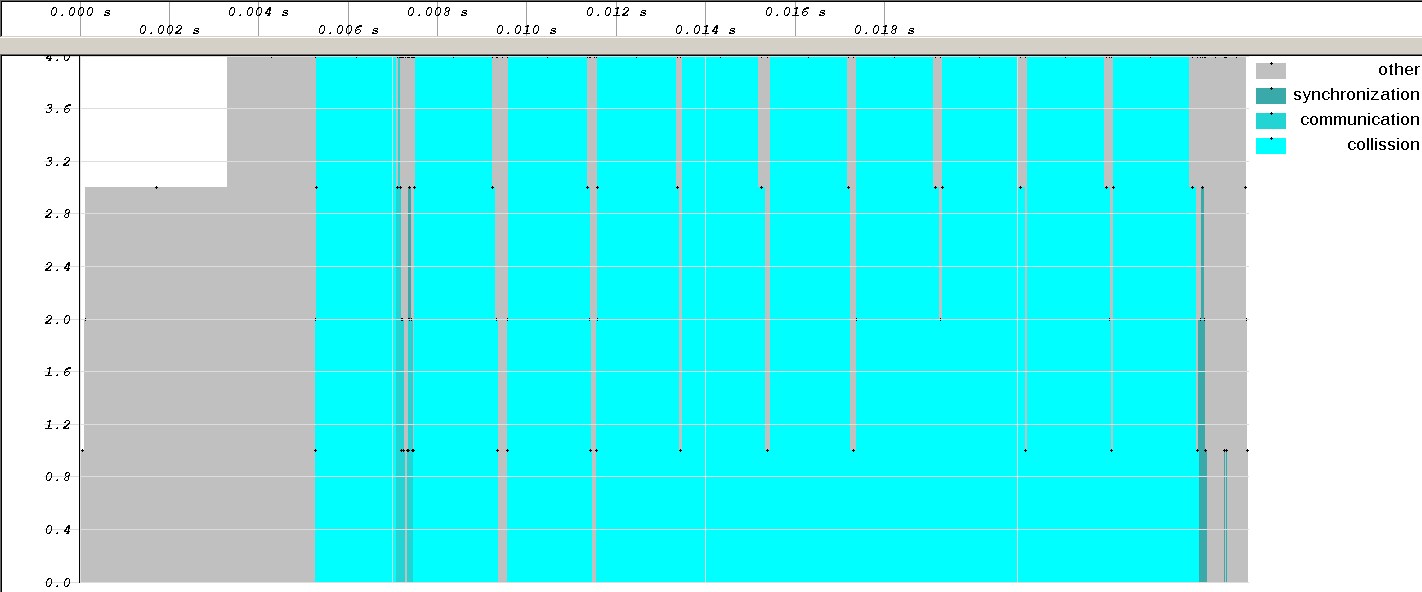
\includegraphics[scale=0.3]{global_timeline.png}
  \caption{Global timeline showing usage of the different groups over time}
  \label{timeline}
\end{figure}

\begin{figure}[H]
  \centering
  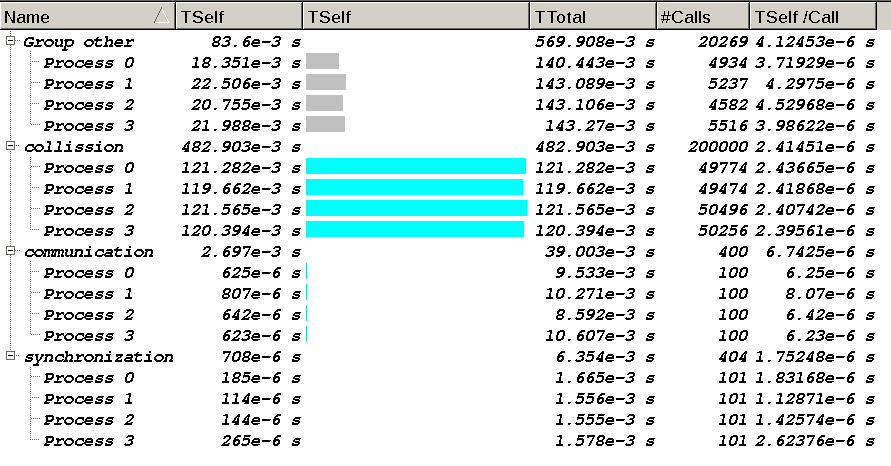
\includegraphics[scale=0.5]{group_times.png}
  \caption{Time spent in the different groups, for each node}
  \label{time}
\end{figure}

\begin{figure}[H]
  \centering
  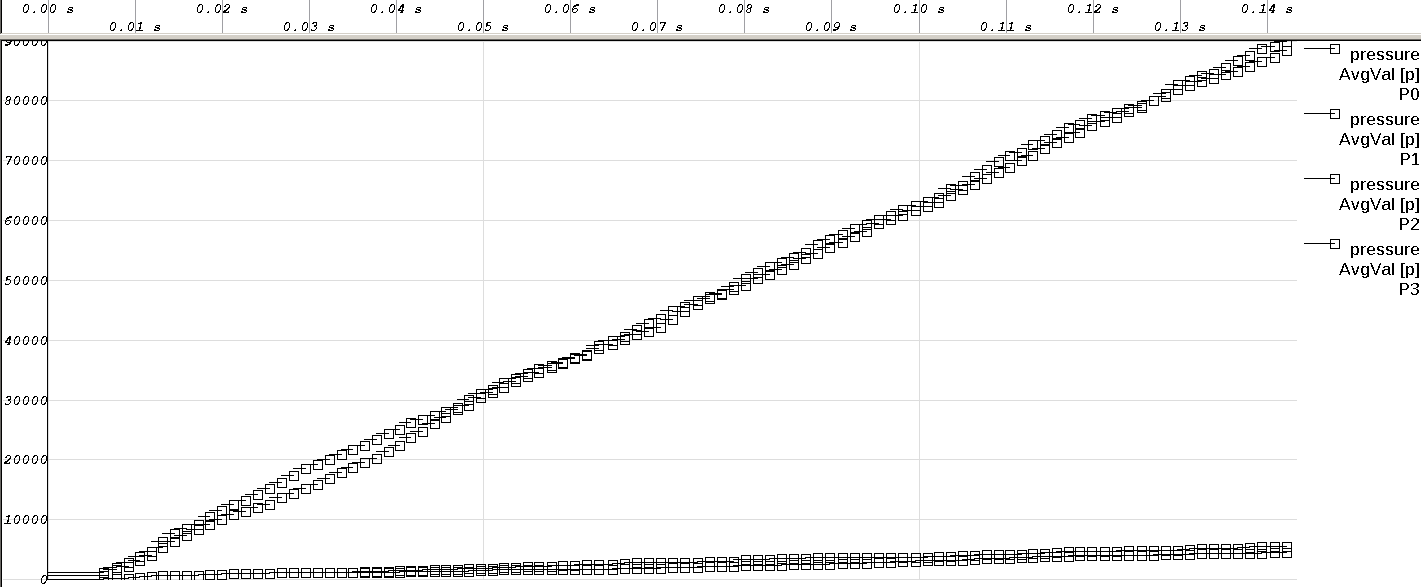
\includegraphics[scale=0.3]{count.png}
  \caption{Count graph of the total momentum for each node}
  \label{count}
\end{figure}


\end{document}
